%bisection diagram

\section{Bisection Diagrams}

\subsection{2-D Bisection of Terminal Triangle Pair}

\begin{figure}
\begin{center}

\vnode{0} \vnode{1} \vnode{2}
\psfrag{vh}{$\widehat{V}$}

\psfrag{longedge}{(longest edge)}

\psfrag{ar1}{\Huge{$\Downarrow$}}
\psfrag{ar2}{\Huge{$\Rightarrow$}}

\psfrag{t0}{$t_0$}
\psfrag{t1}{$t_1$}
\psfrag{s0}{$s_0$}
\psfrag{t0d}{$\tilde{t}_0$}

\psfrag{A}{$A$}
\psfrag{B}{$B$}
\psfrag{C}{$C$}
\psfrag{D}{$D$}

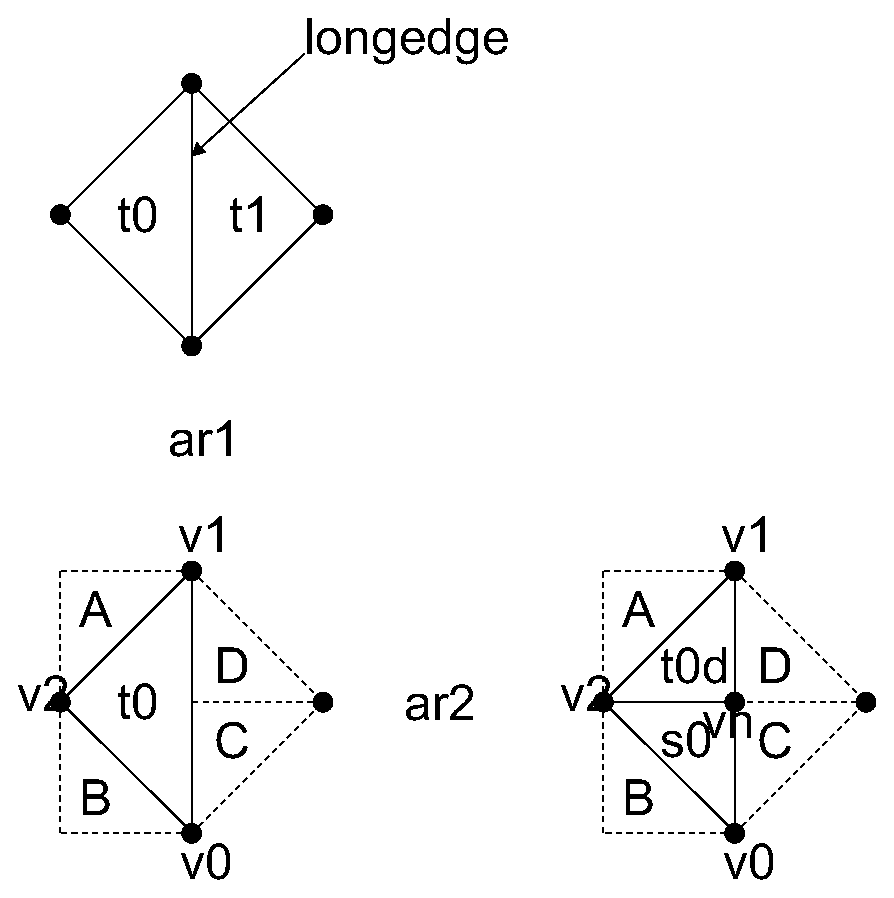
\includegraphics[width=4.0in]{Bisect_Terminal_Triangle_Pair}
\caption{Diagram of bisection process for terminal triangle pair.  The initial pair consists of two triangles $t_0, t_1$ that share a longest edge.  The initial neighbors of $t_0$ are the triangles labeled $A, B, t_1$.  Assuming that $t_1$ has already been bisected into triangles $C, D$, we see an intermediate stage for bisecting $t_0$.  We then replace $t_0$ by triangles $\tilde{t}_0$ and $s_0$ whose neighbors are adjusted accordingly.} \label{fig:Bisect_Terminal_Pair_2D}
\end{center}
\end{figure}

Assume we are given a terminal pair of triangles that share a longest edge (see Figure \ref{fig:Bisect_Terminal_Pair_2D}).  Bisecting the longest edge adds a new vertex with global index denoted $\widehat{V}$.  To better explain the bisection of the adjacent triangles, we assume that $t_1$ is already bisected into two triangles labeled $C, D$.

To bisect the triangle $t_0$, we must replace the triangle connectivity data of $t_0$ with the connectivity data of $\tilde{t}_0$, followed by adding a new triangle to the mesh, namely $s_0$. We then change the neighbors of $t_0$ to those of $\tilde{t}_0$, and add the neighbors of $s_0$ to the neighbor list.  Finally, we adjust the neighbors of $A$ and $B$ to correctly correspond to the new mesh.  This is summarized as follows.
\begin{equation}\label{eqn:tri_connectivity_and_neighbors}
\begin{split}
    \text{triangle~connectivity~of} ~\tilde{t}_0 &= [\widehat{V}, V_1, V_2], \quad \text{neighbor~connectivity~of} ~\tilde{t}_0 = [A, s_0, D] \\
    \text{triangle~connectivity~of} ~s_0 &= [\widehat{V}, V_2, V_0], \quad \text{neighbor~connectivity~of} ~s_0 = [B, C, \tilde{t}_0]
%    \text{neighbor~connectivity~of} ~\tilde{t}_0 &= [A, s_0, D] \\
%    \text{neighbor~connectivity~of} ~s_0 &= [B, C, \tilde{t}_0]
\end{split}
\end{equation}

Note that the global triangle index of $t_0$ and $\tilde{t}_0$ is identical, since we simply \emph{replaced} $t_0$ by $\tilde{t}_0$.  This means that the neighbor data for triangle $A$ does not need to be changed.  However, we must update the neighbors of triangle $B$, i.e. if $B$'s $k$th neighbor was $t_0$ before the bisection, then $B$'s $k$th neighbor after bisection should be $s_0$.

Note: the process for bisecting $t_1$ is exactly the same as for $t_0$; just rotate the diagrams in Figure \ref{fig:Bisect_Terminal_Pair_2D} by $180^\circ$.  In other words, triangle $C$ is really $\tilde{t}_1$, and $D$ is $s_1$.



%%%%%%
